\newpage
\section{Understanding Requirements}
\subsection{Requirements Engineering}
\begin{enumerate}
    \item Inception
    \item Elicitation
    \item Elaboration
    \item Negotiation
    \item Specification
    \item Validation
    \item Requirements Management
\end{enumerate}

\subsection{Building the Analysis Model}
\subsubsection{Elements of the Analysis Model}
\begin{itemize}
    \item Scenario-Based Elements
    \subitem 过家家, 模拟场景
    \item Class-Based Elements
    \item Behavioral Elements
    \item Flow-oriented Elements
\end{itemize}

\subsection{Requirements Monitoring}

\subsection{Validating Requirements}

\section{Requirements Modeling}

\subsection{Scenario-Based Modeling}
\subsubsection{Use Cases}

\begin{figure}[!htb]
    \centering
    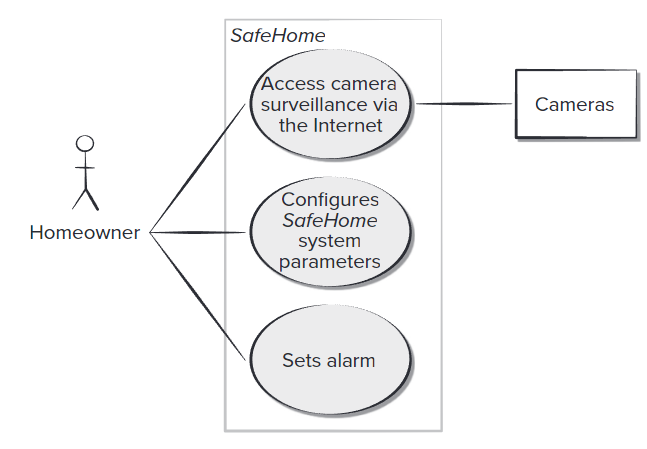
\includegraphics[width=0.309\textwidth]{pic/SE4/use case diagram}
    \caption{use case diagram}
\end{figure}

\subsection{Class-Based Modeling}

\subsubsection{Class Type}
\begin{itemize}
    \item Entity Classes: 自己有的
    \item Boundary Classes: 提供给用户的界面
    \item Controller Classes: 
\end{itemize}

\subsubsection{UML Class Models}
\begin{figure}[!htb]
    \centering
    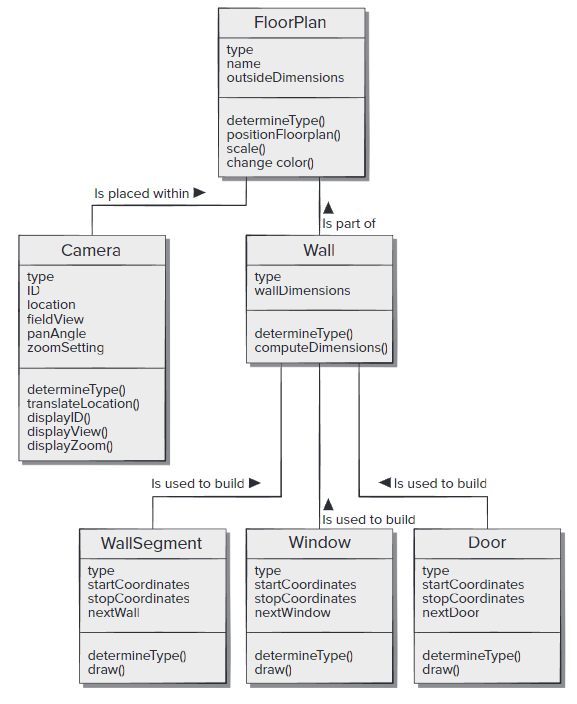
\includegraphics[width=0.309\textwidth]{pic/SE4/UML}
    \caption{UML}
\end{figure}


\subsubsection{Class-Responsibility-Collaborator Modeling}
\begin{itemize}
    \item Classes
    \item Responsibilities
    \item Collaborations
\end{itemize}

\begin{figure}[!htb]
    \centering
    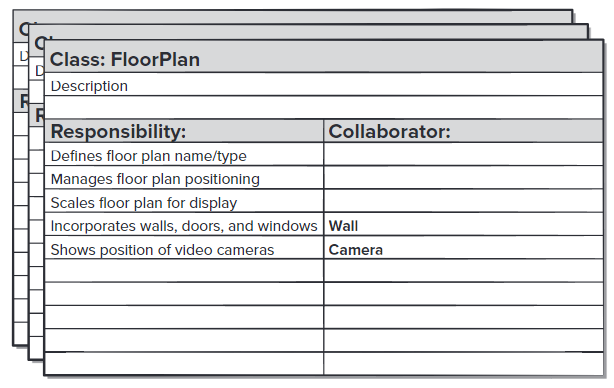
\includegraphics[width=0.42\textwidth]{pic/SE4/A CRC model index card}
    \caption{A CRC model index card}
\end{figure}

\subsection{Behavioral Modeling}
